\chapter{Background}

\section{Citizen Science}

A citizen scientist is ``a volunteer who collects and/or processes data as part of a scientific enquiry." \cite{silvertown2009new} The roots of citizen science date back to the beginnings of modern scientific exploration, where two centuries ago, science was primarily performed as a hobby \cite{silvertown2009new}. With modern communication and the Internet, the number of potential citizens available to do science has grown drastically. Guidelines for scientific research still apply to citizen science projects: the data collected must be validated, the methods of collecting data must be standardized, and volunteers must receive feedback on their contribution \cite{silvertown2009new}.

Citizen science projects have had remarkable success in advancing scientific knowledge \cite{bonney2009citizen}, especially in the bioscience community. These projects often fall into two categories: obtaining data to study large-scale patterns across nature \cite{bonney2009citizen}, or using citizens ability to analyze researcher-collected data that is computationally expensive \cite{cooper2010challenge} \cite{canthepower} or simply too difficult for computers to complete accurately \cite{milkyway2014}.

\subsection{Games With a Purpose}

There are tasks which are trivial for humans but continue to challenge sophisticated computer programs. Traditional approaches to solving this problem focus on improving artificial intelligence systems \cite{gwap}. ``Games with a purpose" \cite{gwap} advocate the constructive channeling of human brainpower through computer games. The Google Image Labeler \cite{googleimagelabeler} is an example of a game with a purpose where users provide meaningful labels to images on the internet, but the game is also fast-paced and competitive. Many games with a purpose avoid using computer vision techniques that do not work well and instead present players with a form of entertainment. ``People play not because they are personally interested in solving an instance of a computational problem, but because they wish to be entertained." \cite{gwap}

The authors presenting ``games with a purpose" propose that the most important aspect of these games is that they are entertaining \cite{gwap}. Even small changes and modifications of the user interface design could influence the enjoyability of these games. The primary objective of games with a purpose is to generate results, whatever they may be. In game with a purpose, throughput could be defined as the number of game objectives completed per human-hour. Games with a higher throughput should be preferred, but it is important that a game is ``fun" as well \cite{gwap}. No matter how efficiently players can solve a game with a purpose, ``fun" is what convinces players to continue playing.

\section{Games}

\begin{quote}
Games are a nascent and complex medium, one which incorporates many previous forms. A single game might include painting, music, cinematography, writing and animation. If that weren’t enough, video games represent an unprecedented collaboration between creator and consumer. We abdicate authorial control to our players and get … something. We’re not quite sure what yet, but we know that it has potential. To many, interactivity seems to be the most important medium of the 21st century. \cite{swink2009game}
\end{quote}

Video games, like the hardware they exist on, have evolved significantly since their birth. More powerful hardware have engaged players with a complex mixture of audio, video, and tactile experiences \cite{atanasov}. Video games are an interesting medium of expression because they encompass so many aspects from a variety of disciplines. Artist disciplines like graphic design, animation, and sound design are expressed with more technical disciplines like computer graphics and computer science concepts. Unlike specifically broadcast mediums like radio, television, newspaper, or books, video games have an added layer of interactivity \cite{schell2008art}.

Designers of novels, television, and other linear entertainment all stress the importance of user experience \cite{schell2008art}. Readers of novels do not influence the experience of the novel, but the novel instead controls the experience. In video games, the distinction betwen the game itself and the experience is much clearer because there is more control by the player \cite{schell2008art}. The player can control which events happen, the pace of the events, and the randomness they may encounter. Feedback is important in games because it reinforces clues about what effects the player's input have.

\begin{figure}
\centering
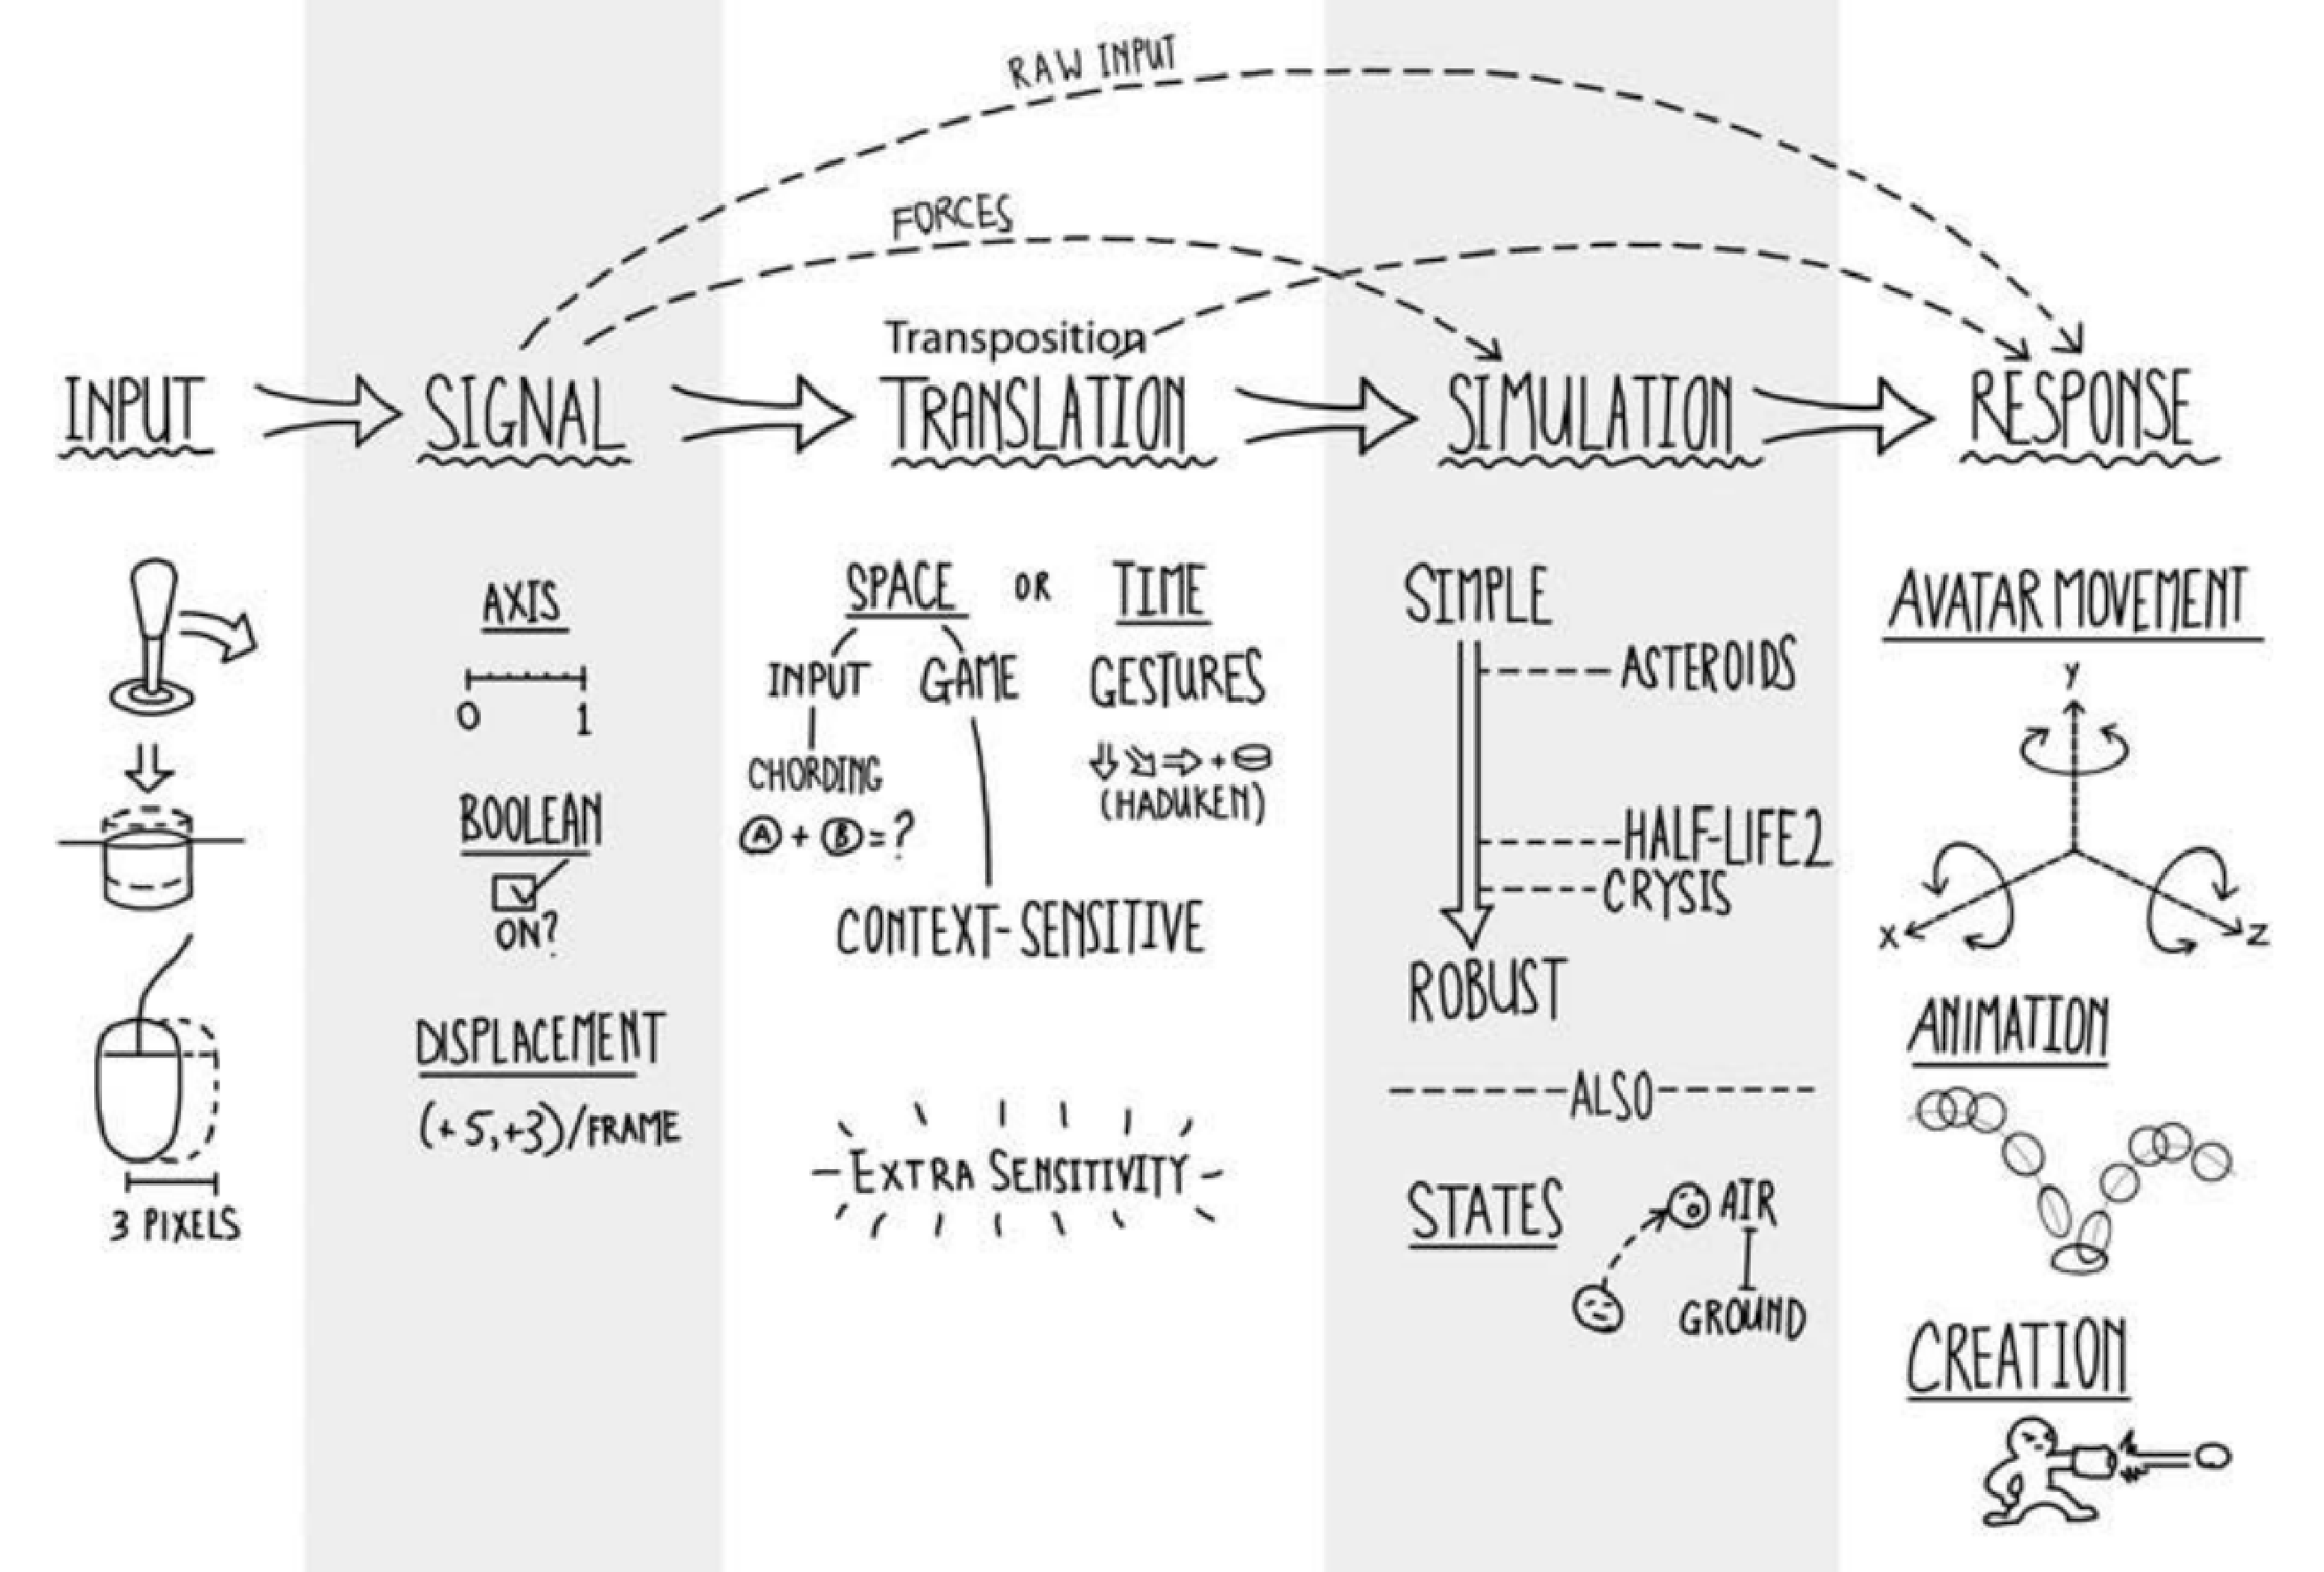
\includegraphics[width=100mm]{images/relationships.pdf}
\caption{The tight relationship between user input and system output is the foundation of great game experience}
\label{fig:relationships}
\end{figure}

While video games are interactive, it's important to note that they, like television or novels, are a tool. They are a means to an experience, Schell is very clear that the experience is completely separate from the game itself \cite{schell2008art}. It is easy to say that the game is the experience because it is real and it exists. The player and game are real, but the experience is imaginary and all games are judged by the quality of this experience because it is the reason that people play games \cite{schell2008art}.

Unfortunately for designers, there is no silver bullet of design. Psychology itself focuses on the measurable, repeatable, controlled results of experimentation but treats the mind as a black box \cite{schell2008art}. There is no objective way to design a game that exhibits a specific experience. Makers of video games (or any entertainment for that matter) can only focus on what seems to be true as opposed to what is definitely true \cite{schell2008art}.

\section{Aesthetics}

``Visceral design is the difference between a high aesthetic design and one that feels infused with soul." \cite{brown2013how} Game and mobile app designers heavily depend on visceral design to create experiences that resonate with the player \cite{brown2013how}. It's about making connections that just ``feel" right. It isn't about just one design choice or mechanic, but a series of overarching interface decisions that acheives a feeling of contentment \cite{brown2013how}. According to the authors, the key to creating visceral design is to focus on feedback loops and essential user flow mechanisms \cite{brown2013how}.

Donald Norman's seminal book, The Design of Everyday Things, proclaims that the most pleasure is attributed to extreme usability \cite{norman2002design}. Later, in Emotional Design, Norman admits that aesthetics create an emotion as essential to the user experience as extreme usability \cite{norman2007emotional}.

Donald Norman breaks aesthetics into three design paradigms: visceral, behavioral, and reflective design \cite{norman2007emotional}. Visceral emotions are the lowest level of emotion--quick judgements that determine whether an experience is good or bad, safe or dangerous. Next, the behavioral level interprets experiences as they happen, whether they are pleasurable and effective. Finally, Reflective emotion is the feeling of self-image and satisfaction that one perceives when remembering an experience. Visceral design can most easily be mapped to appearance, behavioral design to the pleasure and effectiveness of use, and reflective design to the self-image, personal satisfaction, or memories created \cite{norman2007emotional}.

These three designs directly influence human emotion and cognition, which Norman continues to describe as inseperable \cite{norman2007emotional}. Aesthetically pleasing objects enable one to perform better. Scientific studies have again and again refined logical choices and explanations while very few take emotion into account \cite{norman2007emotional}. Norman argues that cognition, the logical, rational side of the brain has equal importance with emotion, or how you feel, how you behave, and how you think. Norman says, ``Emotion makes you smart. Emotion is always passing judgments, presenting you with immediate information about the world. Here is potential danger, there is potential comfort; this is nice, that is bad." \cite{norman2007emotional} The cognitive and the affective sides of the brain work together to determine one's satisfaction of a situation. ``The cognitive side interprets and makes sense of the world around you while emotions allow you to make quick decisions about it." \cite{norman2007emotional}

\section{Game Feel}

``The aesthetic sensation of control is the starting experience of game feel." \cite{swink2009game} This is the pure feeling of enjoying interacting with an interface and having it respond to input---the visceral design component. Experiencing game feel as skill is the process of leanring. This is why some controls feel intuitive and why some control schemes are easier to learn than others.

Game feel is positive feedback from the experience of video games \cite{swink2009game}. Even as game designers, there is no agreed upon defintion for the language to describe game feel. A ``good-feeling" game is one that let's players do what they want without requiring extensive throught process. ``It is to video games what exists in external activities--the aethetics of driving cars, riding bikes, and so on--but nowhere is it so refined, pure, and malleable." \cite{swink2009game}

Game feel is composed from three parts: real-time control, simulated space, and polish \cite{swink2009game}. These ``building blocks of game feel" translate interactions in to experiences. Figure \ref{fig:blocks} demonstrates the connections between these concepts. 

Real-time control is a specific system of interactive where the player intent is transformed into action which the player interprests from the systems output. The user can then percieve the changes and formulate a new action. As players interact with a game in real-time, the correction cycle compares a users actions with the perceptions of changes in the game world. As a player intends to complete an action, they use the games controls and measure the effects to understand how to reach their goal. The correction cycle in figure \ref{fig:correction} separates the levels of intent in real-time control systems \cite{swink2009game}. Though players have a final goal of finding the princess, the correction cycle operates on the level of the avatar moving through the game world. 

Simulated space refers simulated physical interactions in virtual space, perceived actively by the player \cite{swink2009game}. These interactions give meaning and context to the motion and physicality of the objects in space. Players interacting in a simulated space feel that their actions have consequences. They are a frame of reference and gives us the tactile, physical sense of interacting with virtual environments in the same way we interact with our everyday physical spaces. When a player intends to complete an action in the game, a simulated space returns immediate feedback of their action.

Polish refers to the impacts of animations, sounds, particles, and camera shake. These important effects give clues about what type of interaction we are having with game elements and what physical characteristics they are assuming \cite{swink2009game}. Polish is an effect which emphasize or bring clarity to the underlying simulation. Polish effects are only effects that artificially enchance interactions in the game without modifying the underlying simulation and control. Examples are particle effects, crashing sounds as cars collide, camera shake to emphasize a weighty impact. ``This is separate from interactions such as collisions, which feed back into the underlying simulation." \cite{swink2009game}

Many different polish effects can enhance the perception of the game interaction \cite{swink2009game}. ``Juicy" game design borrows heavily from this definition of polish.

\begin{figure}
\centering
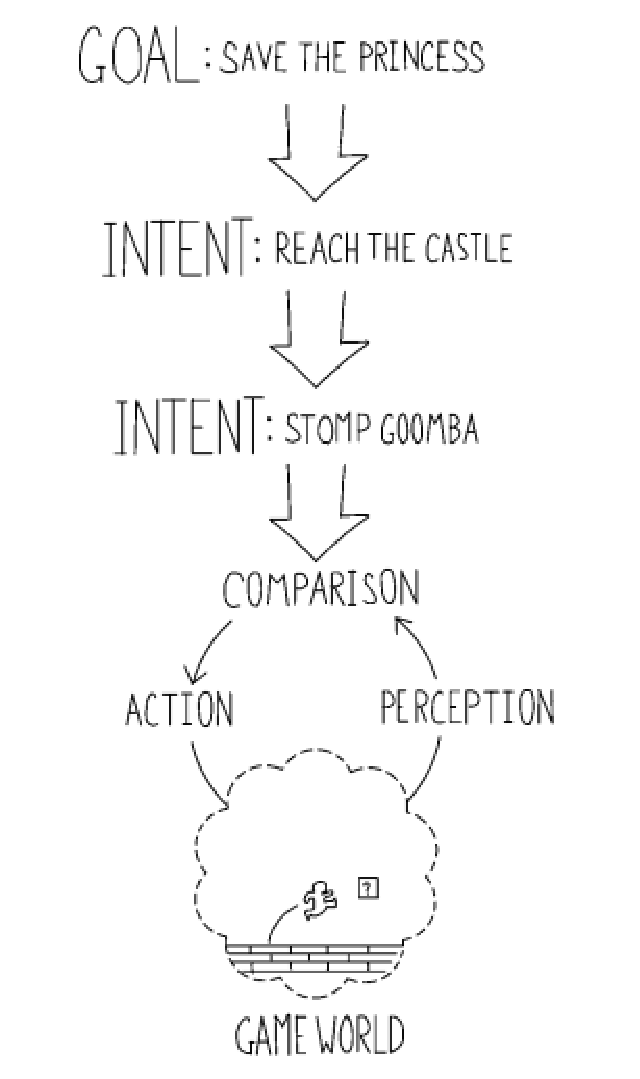
\includegraphics[width=50mm]{images/correction.pdf}
\caption{The correction cycle separates the levels of intent in real-time control systems}
\label{fig:correction}
\end{figure}

\begin{figure}
\centering
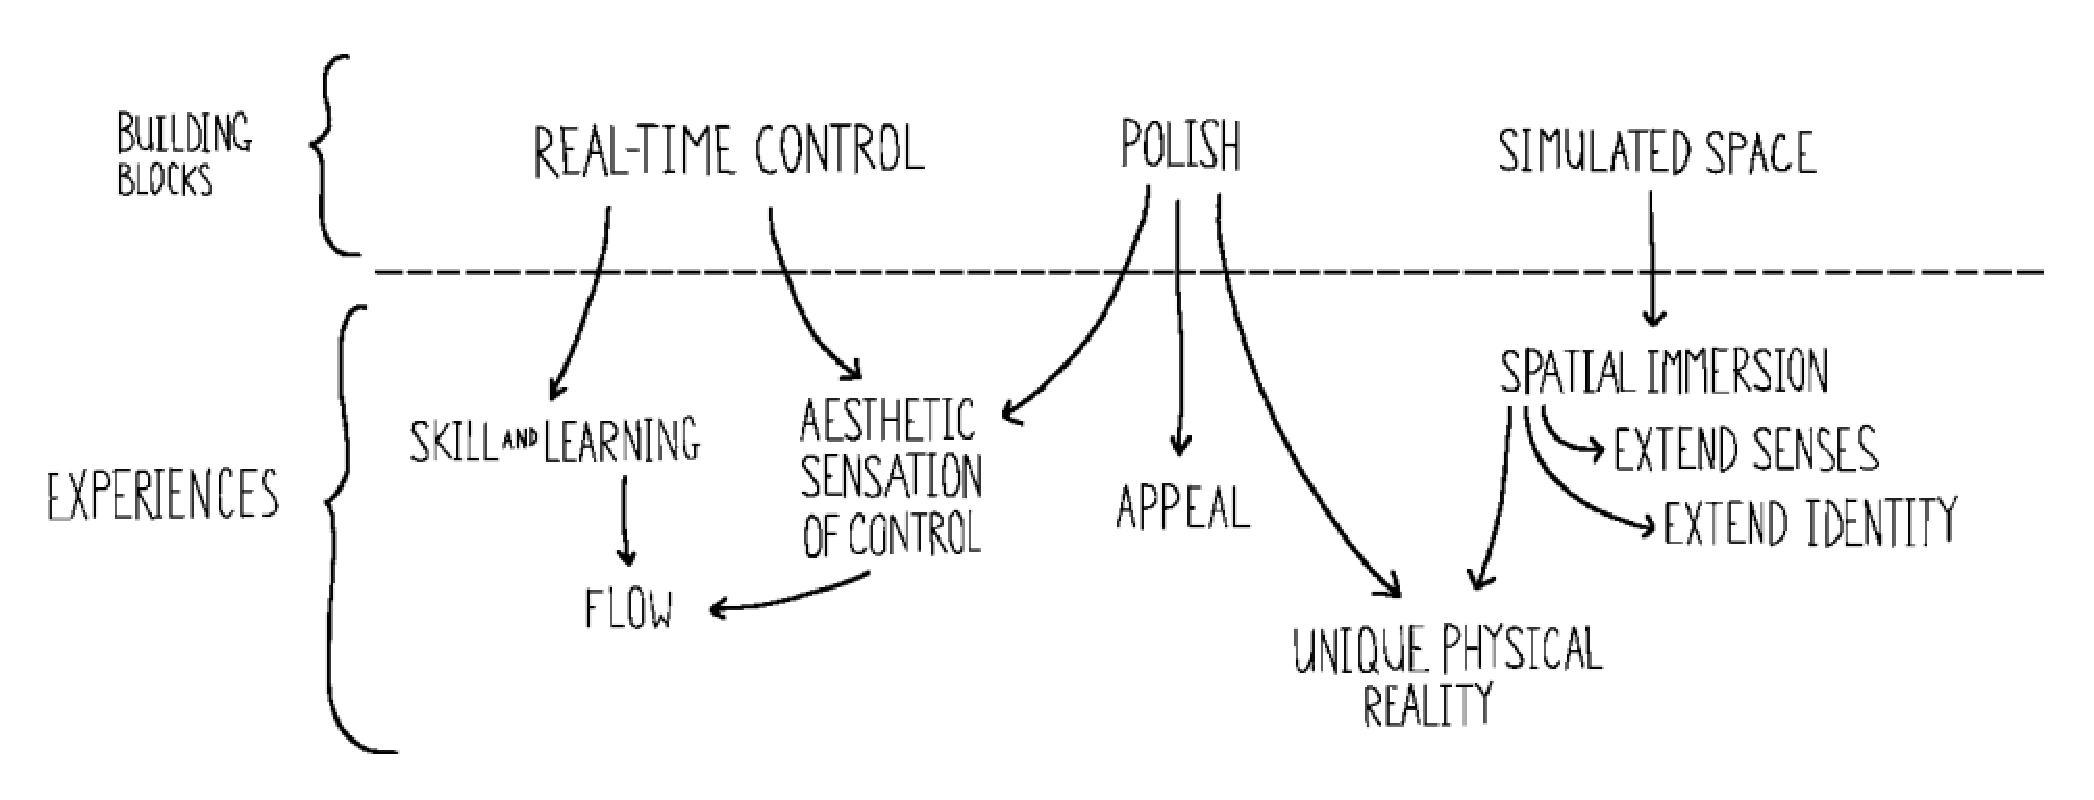
\includegraphics[width=150mm]{images/blocks.pdf}
\caption{Translating game feel into experiences}
\label{fig:blocks}
\end{figure}

\section{Juiciness}

From an influential article published in Gamasutra, ``A `juicy' game feels alive and responds to everything you do--tons of cascading action and response for minimal user input. It makes the user feel powerful and in control of the world, and it coaches them through the rules of the game by constantly letting them know on a per-interaction basis how they are doing." \cite{gamasutra}

The goal of ``juicy" effects is to convey some property about an object or game state by offering feedback clues about how that object interacts with other objects, user input, or its environment. ``Juicy" effects create the difference between a scene of a car starting from stratch and gaining speed and a car screeching and kicking up dust as it speeds away. The car may accelerate at the exact same pace in the two scenarios, but one is loaded with ``juicy" effects that enhance the perception of the experience.

``Juicy" design is aesthetics as much as it is about the experience of playing. Games like Peggle and Bejeweled hark back to the audio-visual bleeps, bloops, flashes of original arcade games, and ``it has to be immediate." \cite{popcap2012} When you're doing well in a ``juicy" game, you don't need to keep your eyes on the score--the game is rewarding you directly through the feedback loop. ``It's not about manipulating behavior, it's about rewarding the stuff that's good for game progress." \cite{popcap2012} A ``juicy" game's appeal doesn't end if when the player reaches the end--simply experiencing the game is fun.

\begin{figure}
\begin{center}
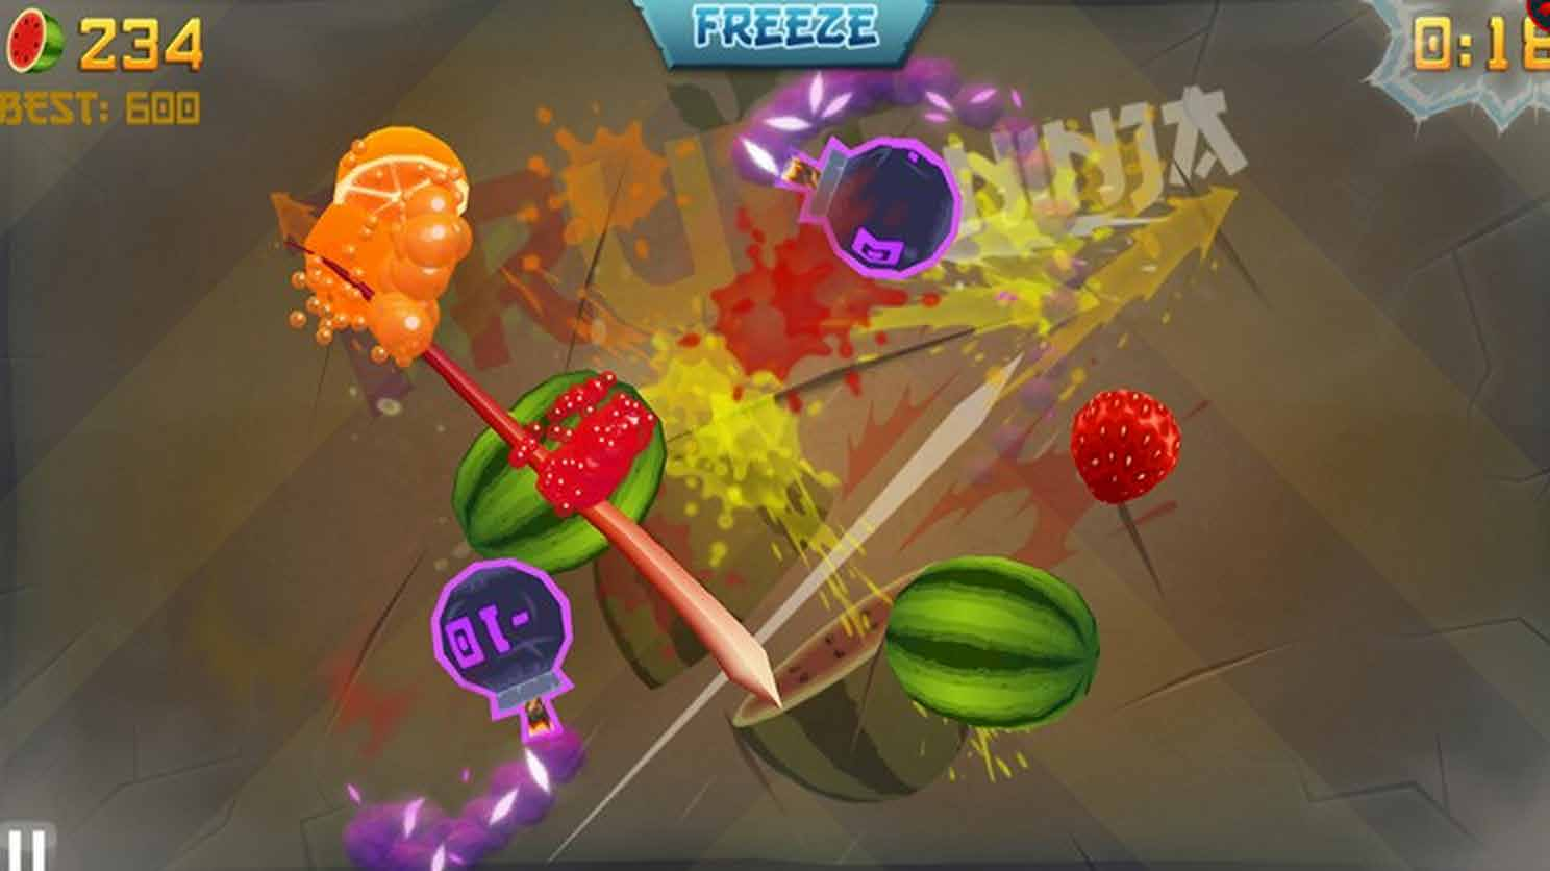
\includegraphics[width=80mm]{images/ninja.pdf}
\caption{With one slice of Fruit Ninja, fruit sections, pulp, juice, and particles all exhibit second order motion}
\label{fig:ninja}
\end{center}
\end{figure}

``Juicy systems reward the player many ways at once. When I give the player a reward, how many ways am I simutaneously rewarding them? Can I find more ways?" \cite{schell2008art} The interface is meant to be more than just a means of communication of information, the interface should be alive, engaging, powerful, and interesting. ``Juicy" interfaces often exhibit plenty of second order motion; that is, motion that is derived from the action of the player." \cite{schell2008art} When you move your finger across the touch-based ``Fruit Ninja", your finger turns into the sharpest knife in the world without a visual representation of a knife. In figure \ref{fig:ninja}, sections of fruit fly in opposite direction and fruit pulp splatters on the wall in a ``juicy" display of second order motion. 

The user deserves to play and explore the possibilites in the ``juicy" interface whereas the ``dry" interface quickly becomes a chore. ``Juiciness" is the combination of satisfaction and empowerment contributing to an overall positive experience \cite{atanasov}.


\subsection{Animation}

\begin{figure}
\begin{center}
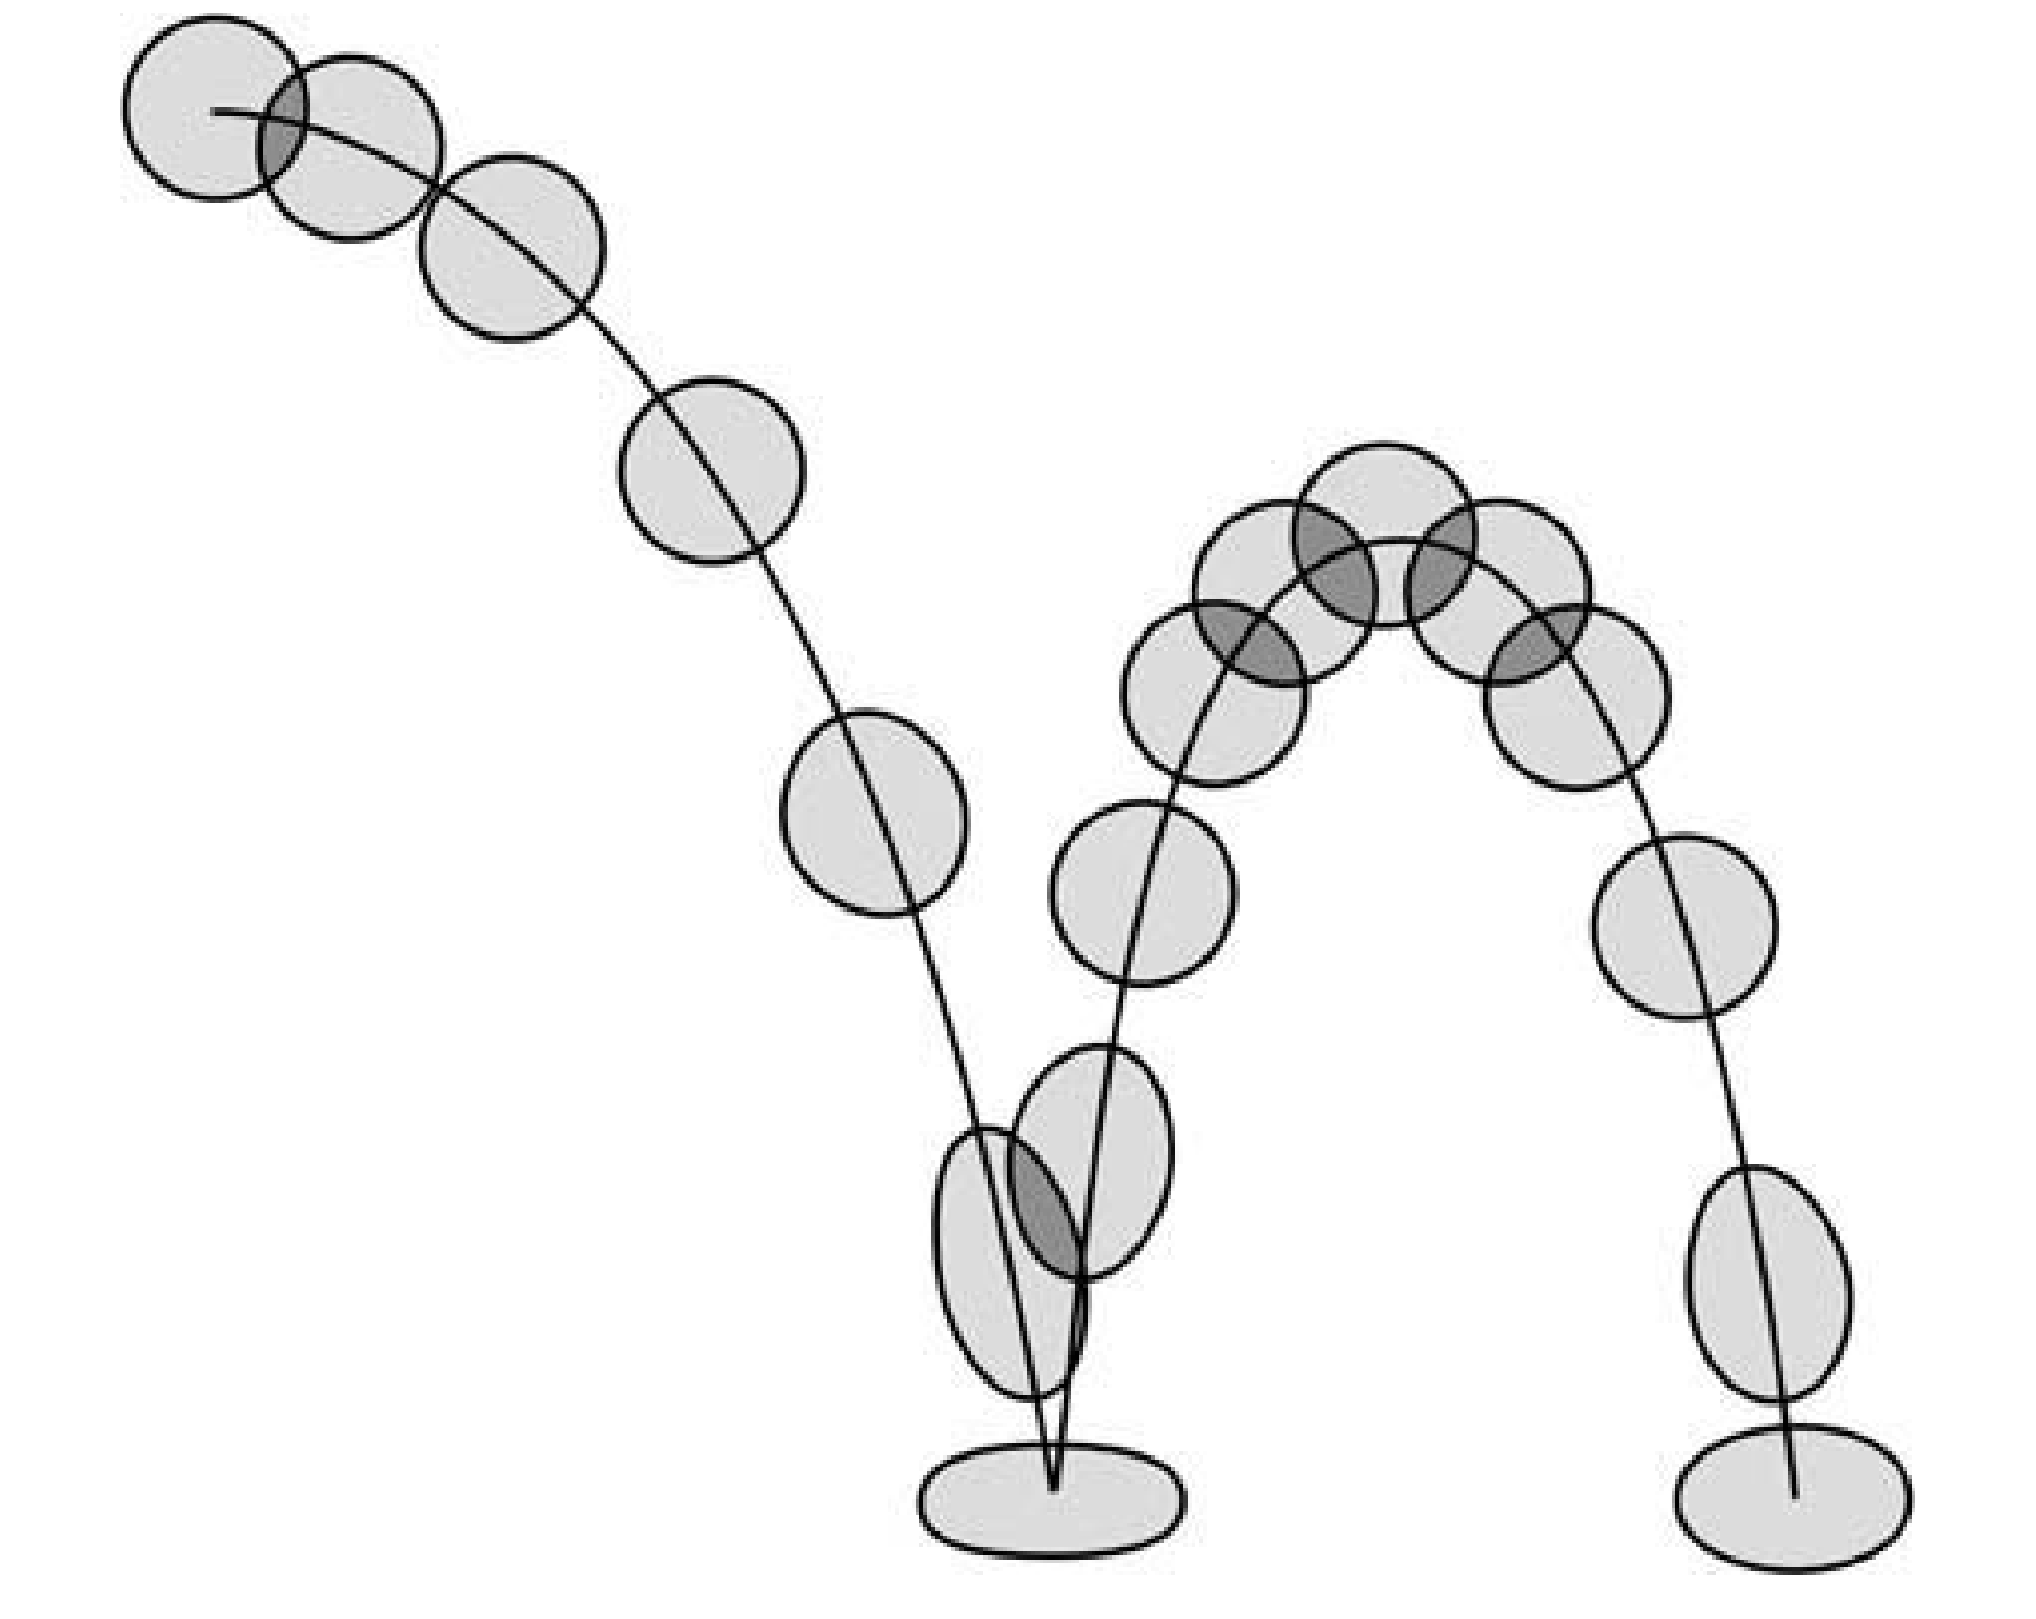
\includegraphics[width=80mm]{images/bounce.pdf}
\caption{The changing shape of the ball as it bounces creates a realistic perception of a bouncing ball, even though the animation doesn’t directly emulate a bouncing ball}
\label{fig:bounce}
\end{center}
\end{figure}

The basic ``principles of animation" were developed by the original animators of Walt Disney Studio, Frank Thomas and Ollie Johnston, during the 1930s \cite{thomas1981disney}. The ``principles of animation" originated the widespread use of concepts like ``squashing and stretching", ``slow in and slow out", ``exaggeration", and ``appeal". 

``Squashing and stretching" gives the illusion of weight and volume to a particular animated effect. It illustrates something fascinating about animation--it is much more believable to exaggerate animations rather than attempting to perfectly replicate real physical properties \cite{swink2009game}. For example, when the bouncing ball animation reaches the ground, viewers are convinced and interested when the ball squishes to almost nothing at the bottom proceeded by stretching when the ball is mid-air. Martin Jonasson uses squashing and stretching as a subtle effect to give life to collisions and interactions in their breakout game \cite{juiceitorloseit}.

\subsubsection{Tweening}

``Slow in and slow out" refers to a specific type of animation that attempts to model accelerations and decelleration. Short for inbetweening, ``tweening" is the process of generating animation frames between two states, giving the appearence of evolution from one state to the next. The process dates back to traditional animation when the head animator would draw the keyframes and have the inbetween frames completed by their assistant. Computer animators use tweening to complete animation between certain desired key frames in animation, or certain states in game design. Tweening is a function of translation over time of a scalar, but vectors can be broken down into multiple scalar values \cite{penner2002robert}. As Martin Jonasson states, ``you can't always use tweening, but it's dirt easy to implement and it feels luxurious." \cite{juiceitorloseit} Most physical scalar values in ``juicy" video games are ``tweened" in some way.

In the physical world, objects infrequently changes states instantly. Whether the change be translation, rotation, colors, or opacity, tweening gives liveliness to motion and make computer elements interesting to watch. Tweening is perfect for game animation because with the quick change of a tweening function, different elements can exhibit completely transitions invoking a different emotional response to its behavior.

\subsection{Visual Effects}

Where animations dictate how objects move in context of their simulated space, visual effects highlight the interaction between objects \cite{swink2009game}. Usually, visual effects appear only momentarily such as sparks flying off the bottom of a car or a crate shattering into an array of splinters. Visual effects can also be caused by an object, though it is not the animation of the object itself. Many sword fighting games employ this effect. A streak of light will follow a sword to emphasize the speed and strength of the character wielding it. In the ``juicy" breakout clone by Martin Jonasson, screen flashes and shaking are used to emphasize the weight of a collision \cite{juiceitorloseit}.

These effects encompass particle effects too. Particle effects are typically temporary indicators of movement or interaction or a specific quality of an item. Smoke and fireworks are common particle creations, and the motion of the particles is much more important than their color or shape. The motion is how players associate meaning with the particles \cite{swink2009game}.

\subsection{Sound Effects}

Sounds effects are repeatable sounds that players can associate with particular interactions in a game. Often a range of sounds will associate with an interaction to keep the players from hearing the exact same sound over and over \cite{swink2009game}.
